\section{Source Term}
For licensing existing operating reactors a mechanistic source\footnote{Mechanistic Source Term: A source term that is calculated using models and supporting scientific data that simulate the physical and chemical processes that describe the radionuclide inventories and the time-dependent radionuclide transport mechanisms that are necessary and sufficient to predict the source term.}
 is used for the transport of the fission products from the fuel through the reactor coolant system, through all holdup volumes and barriers, taking into account mitigation features, and into the environment. Such a method method to determine accident dose is also under consideration for microRs.  \\
 
The source term is expressed as\\
ST(S$_{i}$, RN$_{j}$, t) = I(RN$_{j}$).F(S$_{i}$, t).MR(S$_{i}$, RN$_{j}$, t).PSR(S$_{i}$, RN$_{j}$, t).LPF(S$_{i}$, RN$_{j}$, t)\\
where,\\
ST(S$_{i}$, RN$_{j}$, t) - Source term as a function of the accident scenario (Si), radionuclide class (RNj), and timing (t)\\
I(RN$_{j}$) - Inventory \\
F(S$_{i}$, t) -Fuel damage\\
MR(S$_{i}$, RN$_{j}$, t) - Matrix release\\
PSR(S$_{i}$, RN$_{j}$, t) - Primary system release\\
LPF(S$_{i}$, RN$_{j}$, t) - Leak path factor\\

As tabulated in Table \ref{inputandsource}, inputs that used in the source term calculation may come from experiments or other computer codes. A general source term analysis comprises transient scenario modeling, fuel pin radionuclide distribution, failed pin radionuclide release, radionuclide bubble transport, offsite dispersion analysis and containment region analysis. Some of them can, however, be eliminated or new ones can be added depending on which micro-reactor is to be chosen. As an example, the micro-reactor design does not include any spent fuel storage, thus the source term would not. \\

\begin{table} [ht]
\begin{center}

\caption{ Inputs used in the source term calculations and their sources}
\label{inputandsource}
\begin{tabular}{l l}
\hline 
Input 		&Source \\ 
\hline 
FP inventory 		&SCALE\\ 
FP diffusion coefficients 		&Experiments and analysis (e.g., DOE tools) \\ 
Core power shape		&Radial/Axial profiles (e.g., SCALE or vendor data)  \\ 
Fuel particle failure rate response surface \\
(function of temperature and burnup)	&Experiments/other codes (e.g., DOE tools) \\ 
Dust generation, lift-off, and FP adsorption on dust \\
(impact of aerosol growth, shape factor, etc.)	& Experiments/Historical data and other codes\\ 
FP release under accident conditions \\including air/water ingress 	&Experiments \\ 
FP speciation and interaction \\with graphite and other structures &Experiments  \\ 
\hline 

\end{tabular}
\end{center}
\end{table}

MicroRs have significantly lower source terms (about 1\% of typical 1000 MWe LWR) due to their reduced fuel inventory and passive safety features. A reduced source term would facilitate siting SMRs in locations where nuclear plants have not been traditionally sited.\\\\
For the source term analysis of a selected micro-reactor design, phenomena and release paths of accident scenarios first need to be identified. Eventhough pathways for some advanced reactors (i.e., HTGR, \gls{SFR}, MSR) illustrated in Fig. \ref{pathway} are known  \cite{inl_htgr_2010}, there are on-going discussions in the NRC on the evaluation of the source term of micro-reactors; it is expected to come to a conclusion on the licencing issues including the source term by the end of this year (estimated). 

\begin{figure}[hbtp]
\centering
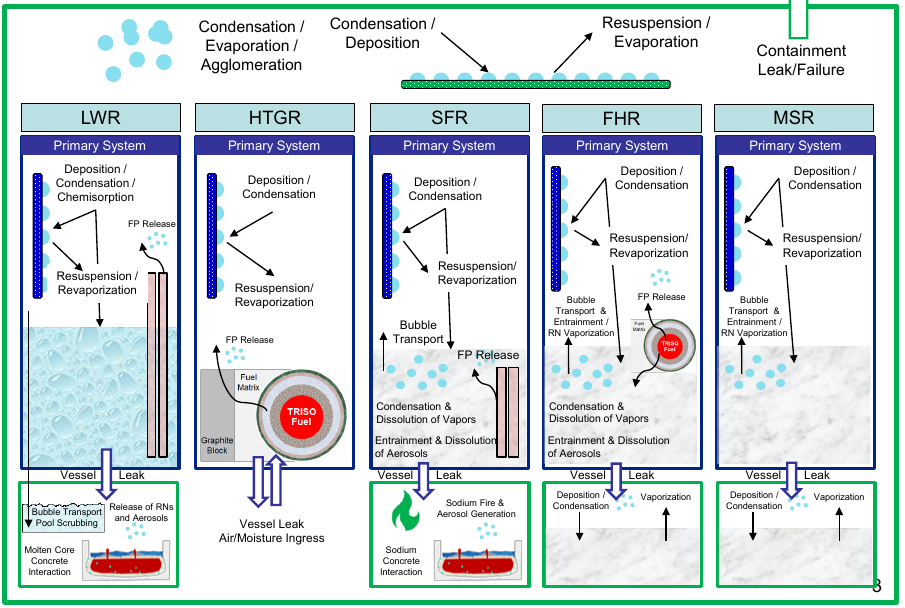
\includegraphics[scale=0.6]{Figs/pathway.jpeg}
\caption{Pathway for radioactive release for several reactor types}
\label{pathway}
\end{figure}

There is a possibility to make an assumption for the pathway identification of the micro-reactors. We can use the same or modified pathways of the existing reactors, accepted by the NRC, for the analogy to the selected micro-reactor design. \\

A recent document by the NRC \cite{nrc_staff_nrc_2019} has published for the source term calculations of non-LWR reactors.
The method for the source term calculation recommended by the NRC is given in Fig. \ref{sourceterm}. The method to be applied changes with the type of the reactor. In any cases, as a code system, SCALE calculates radioactive material composition for the licensed current and advanced reactors and provides necessary data to MELCOR. MELCOR, system accident analysis code, produce the source term for the defined design-basis accidents. And then, for probabilistic offsite consequence analysis bounded by the calculated source term, MACCS code needs to be utilized. The code is capable of evaluating the Level 3 \gls{PRA} including the radionuclide release, atmospheric transport, meteorology, protective actions, site data, dosimetry, health effects, economic factors, and so forth. Design-specific and site-related issues must be input to the code.  Meteorological statistics (i.e., day and night temperatures, magnitude and direction of the wind, tornados, flooding level), topographical data and population density and distribution, habitat of the animals and the location of the endemic plants are to be recorded. \\

The methodology and the results on the source term calculations are presented in detail in the relevant documents of NuScale \cite{nuscale_chapter_2018-1} and eVinci \cite{maioli_westinghouse_2019}.According to the NuScale, the potential radionuclide source term associated with a severe accident is much smaller (5\%) than that associated with a 1000 MWe design. This value is 1\% for eVinci. 

\begin{figure}[hbtp]
\centering
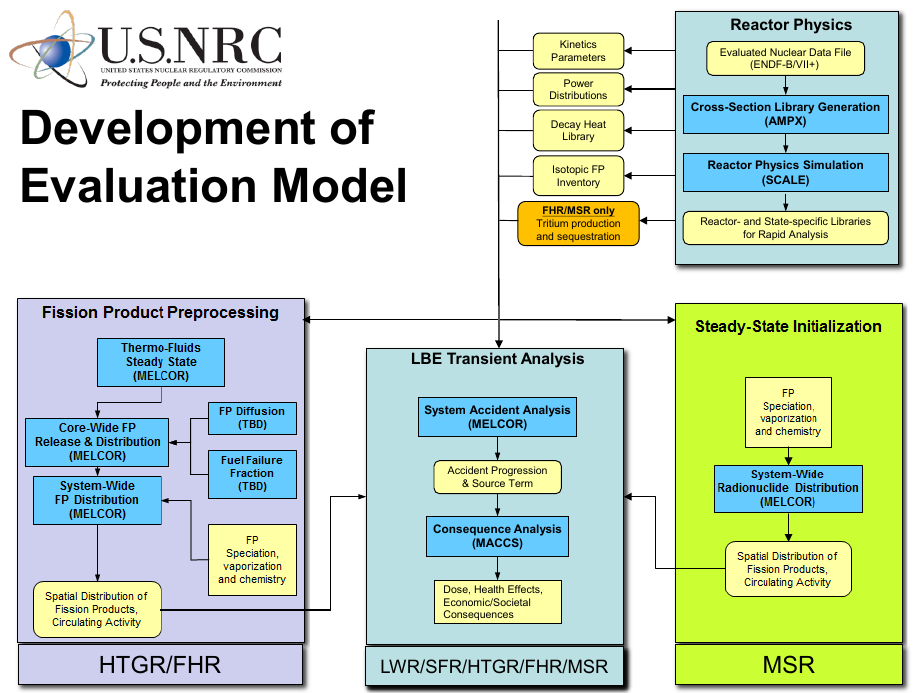
\includegraphics[scale=0.6]{Figs/sourceterm.jpeg}
\caption{Source term evaluation model}
\label{sourceterm}
\end{figure}

\subsection{HTGR}
Pathway for HTGR is given in the reference  \cite{inl_htgr_2010}. There is a generic pathway almost for all HTGRs. NRC evaluation model for HTGRs is displayed in Fig. \ref{sourceterm}. Source term calculation for HTGRs is given in Fig.  \ref{htgrsourceterm}. 

\begin{figure}[hbtp]
\centering
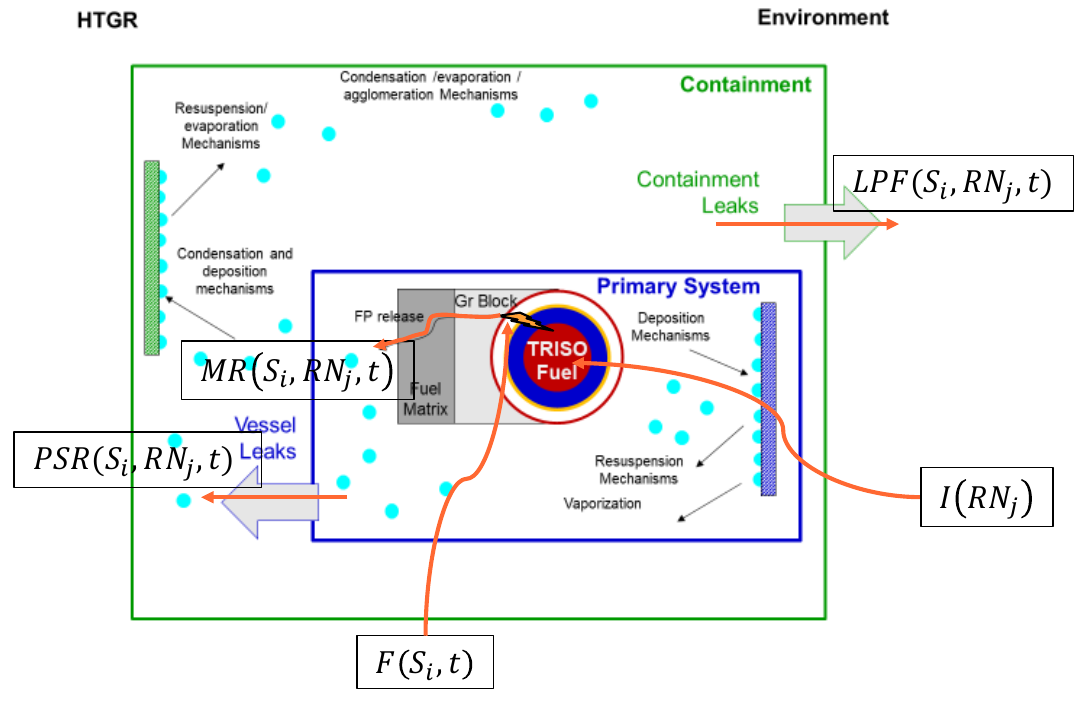
\includegraphics[scale=0.5]{Figs/htgrsourceterm.jpeg}
\caption{Source term calculation for HTGRs}
\label{htgrsourceterm}
\end{figure}

\subsection{Heat Pipe Reactor}
In contrast to HTGRs, pathways for the radioactive material release from the heat pipe reactors are completely unknown. However, source term evaluation model is very similar to HTGRs once the pathway of HPRs is defined.  



